\documentclass[12pt]{article}
   
   \usepackage[utf8]{inputenc}
   \usepackage{graphicx}
   \usepackage{float}
   \usepackage{subcaption}
   %\usepackage{mathtools}
   %\usepackage{amsmath}
   
   \addtolength{\hoffset}{-0.7in}
   \addtolength{\textheight}{1.5in}
   \addtolength{\textwidth}{1.5in}
   \addtolength{\voffset}{-1in}
%
% Title.
\title{EE230: Experiment 2\\
Non-idealities in Op-amps}

% Author
\author{Hitesh Kandala, 180070023}

% begin the document.
\begin{document}

% make a title page.
\maketitle

\section{Overview of the experiment}

\subsection{Aim of the experiment}

In reality, no OpAmps are ideal,they all have some non-idealities which can affect our measurement. Some of these major non-idealities of UA741 Op-amp are:\\ a) Input Offset voltage \\ b) Input Bias currents \\ c) Finite open-loop gain.

\begin{figure}[H]
    \centering
    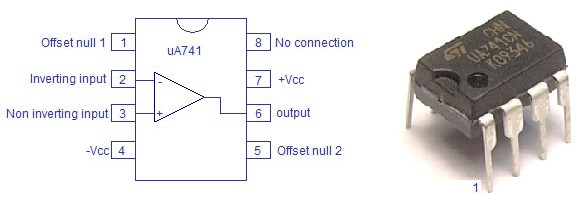
\includegraphics[width = \linewidth, height = 2in]{uA741-pinout.jpg}
    \caption{Pinout and external appearance of Op Amp 741}
\end{figure}

\subsection{Methods}

(i) For measuring the non-idealities such as offset voltage and input bias currents, we design circuits that enhance the contributions one of these parameters while keeping the other two contributions small.
\\
(ii) DC open loop gain is measured in such a way that it actually contributes to the high closed loop gain of the non-inverting amplifier, the circuit is designed considering the appropriate values of resistance such that even the gain is high and op-amp doesn't go in saturation.
\\
(iii) We also measured open loop gain of AC input signal for different frequencies to understand a brief relation of open loop gain with frequency.

\section{Design of Op-amp 741}

        \begin{figure}[H]
            \centering
            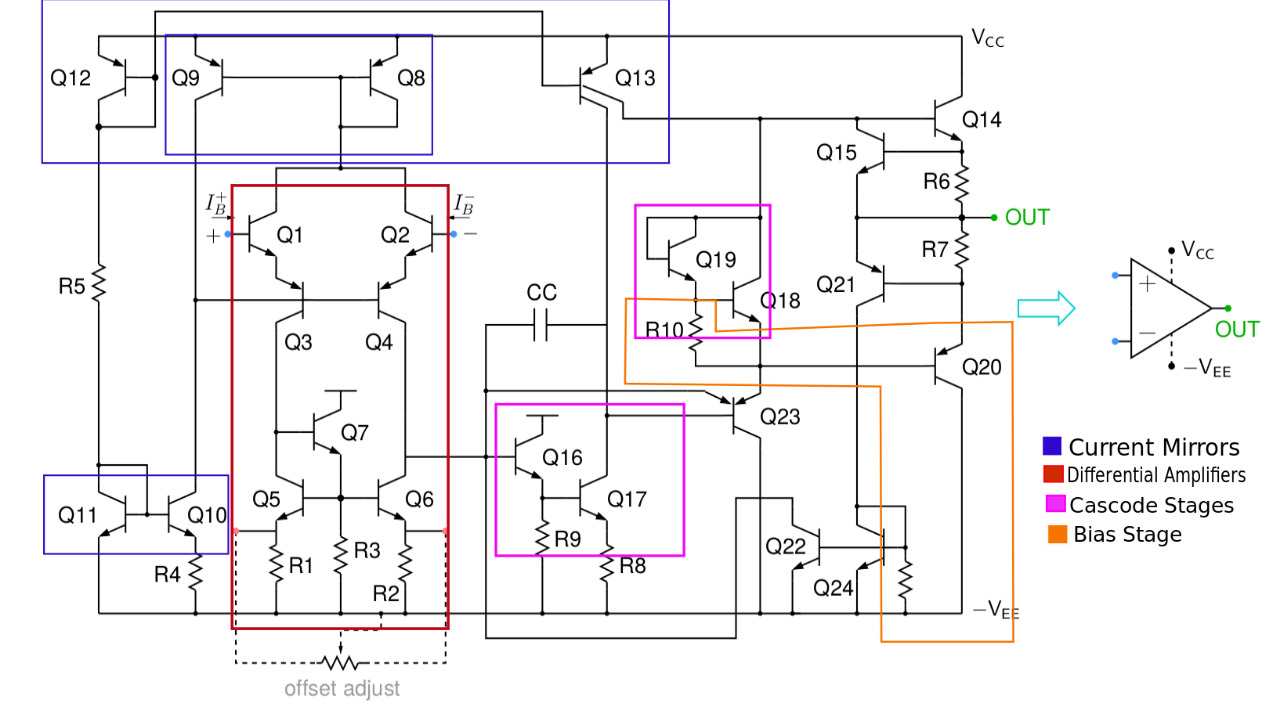
\includegraphics[width = \linewidth, height=5in]{opamp.jpeg}
            \caption{Internal circuit of Op Amp 741}
        \end{figure}
        
\begin{itemize}
    \item The current mirror circuit copies or mirrors the current flowing in one active device in another, keeping the output current constant regardless of loading. An ideal current mirror is simply an ideal inverting current amplifier that reverses the current direction as well or it is a current-controlled current source (CCCS). The current mirror is used to provide bias currents and active loads to circuits.
    \item The differential amplifier amplifies the voltage difference present on its inverting and non-inverting inputs.
    \item A single stage of amplifier can provide only a limited current gain or voltage gain. Therefore for a higher voltage gain or current gain, several amplifier stages are connected in cascade i.e. connected such that the output of one stage becomes the input to the next stage.
\end{itemize}
\newpage
\section{Experimental results}

\subsection{Input offset voltage measurement}
\begin{figure}[H]
            \centering
            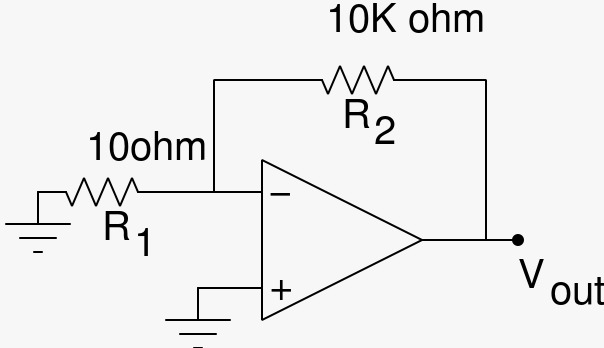
\includegraphics[width = 0.6\linewidth, height = 2in]{offset.jpeg}
            \caption{Cicuit diagram for measuring $V_{OS}$}
        \end{figure}
        
        \begin{figure}[H]
            \centering
            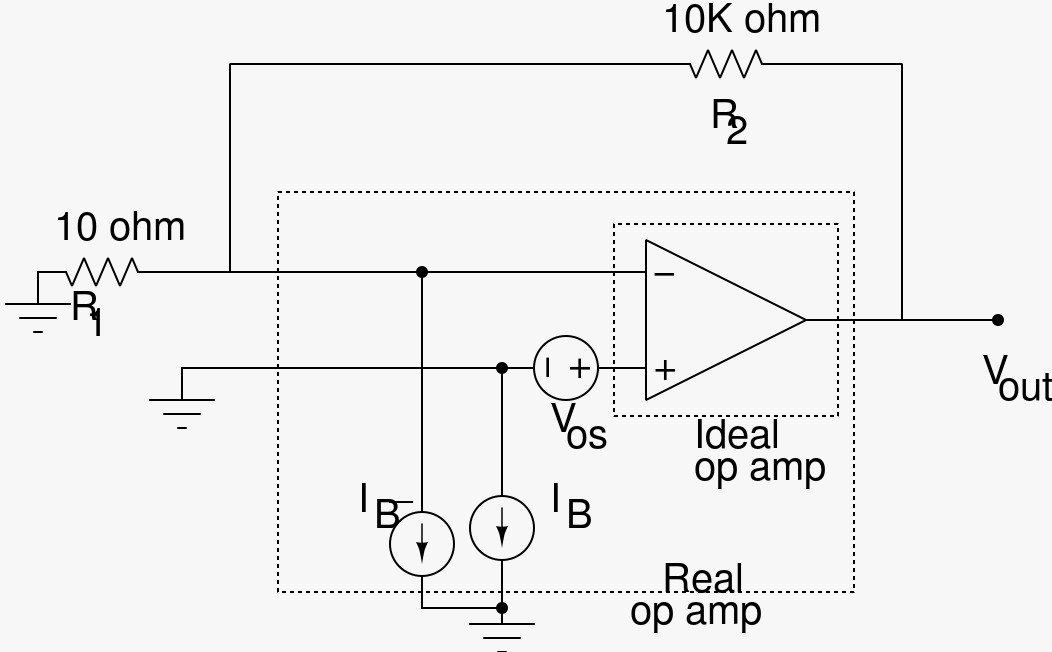
\includegraphics[width = 0.8\linewidth, height = 2.5in]{offset_real.jpeg}
            \caption{Equivalent circuit}
        \end{figure}
\begin{equation}
            V_0 = V_{OS}\left(1 + \frac{R_2}{R_1}\right) + R_2I^-_B 
        \end{equation}
      \\
        By choosing $R_1$ and $R_2$ as given in the circuit, we can neglect the second term in the above equation as $V_{OS} \approx 5mV$ and $I_B \approx 100 nA$. Hence
         
        \begin{equation}
            V_{OS} = \frac{V_0}{1 + \frac{R_2}{R_1}} \approx \frac{V_0}{\frac{R_2}{R_1}}  
        \end{equation}
        \\
        The observed output value for $ua 741$ is  $1.11V$, hence $\mathbf{V_{OS} = 1.11mV}$


\subsection{Bias currents measurement}
      \begin{figure}[H]
            \centering
            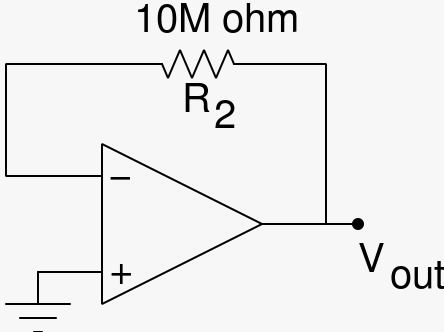
\includegraphics[width = 0.5\linewidth, height = 2.5in]{ibminus.jpeg}
            \caption{Cicuit diagram for measuring I^-_B}
        \end{figure}
        \begin{figure}[H]
            \centering
            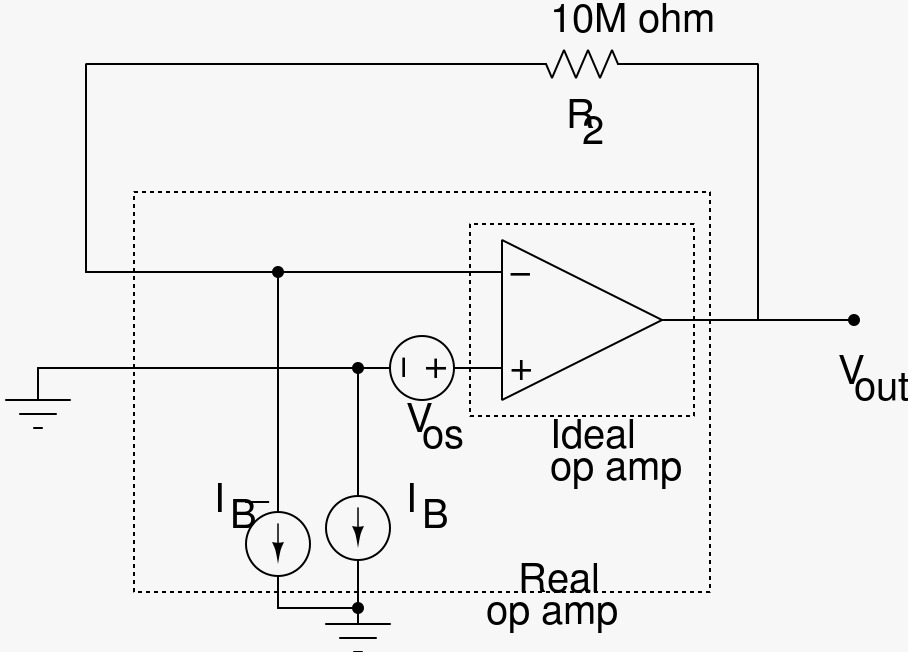
\includegraphics[width = 0.8\linewidth, height = 3in]{ibminusreal.jpeg}
            \caption{Equivalent internal circuit}
        \end{figure}
            \begin{equation}
            V_0 = V_{OS} + RI^-_B
        \end{equation}
        
        R has chosen large so that the second term is large enough to neglect the first term, hence
        
        \begin{equation}
            I^-_B = \frac{V_0}{R}
        \end{equation}
        
        The observed output value for $ua 741$ is  $0.354V$, hence $\mathbf{I^-_B = 35.4nA}$
        \begin{figure}[H]
            \centering
            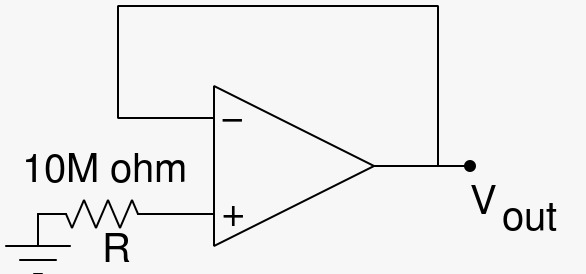
\includegraphics[width = 0.6\linewidth, height = 2.5in]{ibplus.jpeg}
            \caption{Cicuit diagram for measuring I^+_B}
        \end{figure}
        \begin{figure}[H]
            \centering
            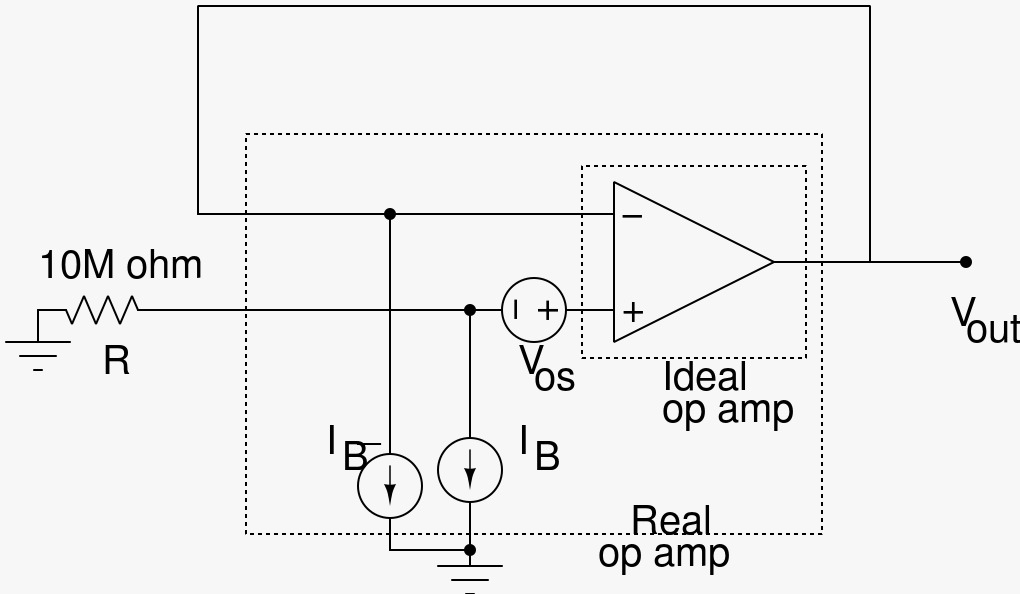
\includegraphics[width = 0.8\linewidth, height = 3in]{ibplusreal.jpeg}
            \caption{Equivalent internal circuit}
        \end{figure}
        \begin{equation}
            V_0 = V_{OS} - RI^+_B
        \end{equation}
        
        Similarly the equation can be approximated to 
        
        \begin{equation}
            I^+_B = -\frac{V_0}{R}
        \end{equation}
        
        The observed output value for $ua 741$ is  $-0.343V$, hence $\mathbf{I^+_B = 34.3nA}$
      
      \subsection{DC open-loop gain measurement}
      \begin{figure}[H]
            \centering
            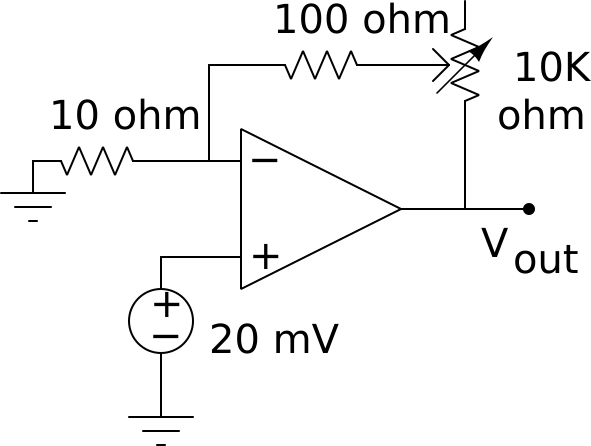
\includegraphics[width = 0.6\linewidth, height = 2.8in]{XC24827.png}
            \caption{Circuit diagram for measuring DC open loop gain}
        \end{figure}
      The actual gain expression for the above circuit is
      \begin{equation}
          Gain = \left(1 + \frac{R_2}{R_1}\right)\frac{1}{1 + \left(1 + \frac{R_2}{R_1}\right)\frac{1}{A_v}} 
      \end{equation}
      
      To find the open loop gain($A_v$), we found the gain for large values of $\left(1 + \frac{R_2}{R_1}\right)$ so that $A_v$ contributes for the actual gain \\
      Also we have taken care of choosing $\left(1 + \frac{R_2}{R_1}\right)$ so that op-amp does not saturate and the actual gain can be measured \\
      
      For $1 + \frac{R_2}{R_1} = 870$ we observed a gain of 663.5 and so $\mathbf{A_v}$ was $\mathbf{2.8\times10^3}$    \\
      
      The challenge we faced in this experiment was finding the feedback resistance as it's a variable resistance, we had to find out the current and the voltage through and across the feedback resistor to find it's resistance along with the output voltage to find the gain. So we ended up with using all the multimeters we have.\\
      
      \textbf{Note:} Instead of nullyfying offset voltage in this experiment using pin 1 and pin 5 of the IC, we included it in the Gain expression. The Gain was adapted to 
      
      \begin{equation}
          Gain = \frac{V_{out}}{V_{in} + V_{OS}}
      \end{equation}
       
\subsection{Variation of open-loop gain with frequency}
        \begin{figure}[H]
            \centering
            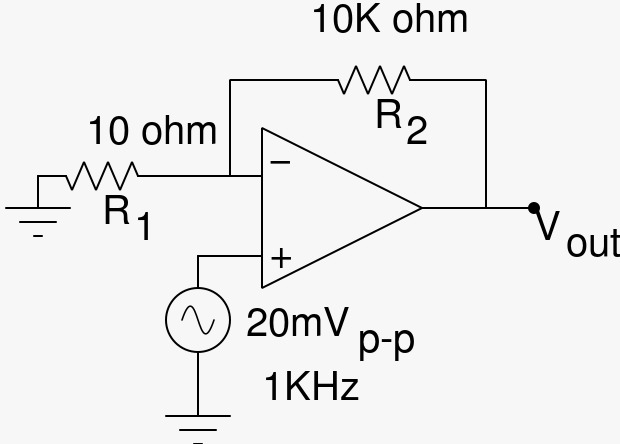
\includegraphics[width = 0.5\linewidth, height = 2.5in]{olg.jpeg}
            \caption{Circuit diagram for measuring open loop gain $A_v$}
        \end{figure}
        \begin{figure}[H]
            \centering
            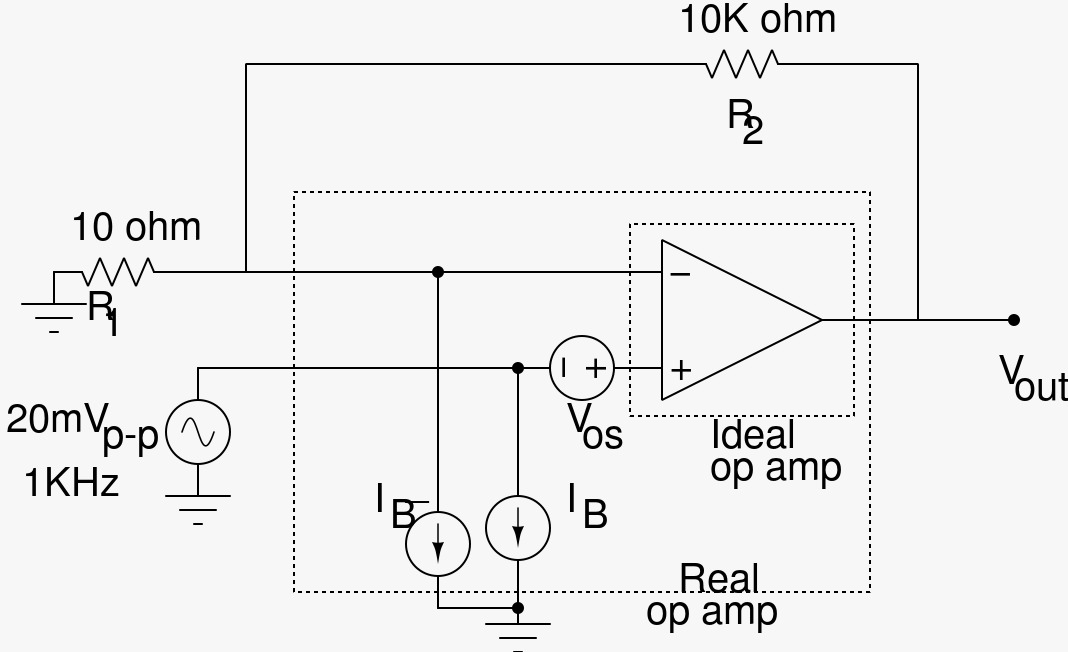
\includegraphics[width = 0.8\linewidth, height = 3in]{olgreal.jpeg}
            \caption{Equivalent internal circuit}
        \end{figure}
      Analysis of open-loop gain with frequency was achieved with AC input which is similar to the previous section with just a change in values of $R_2 = 10K\Omega$ and $R_1 = 10\Omega$ here the closed loop gain was $1000$, the observations were
        
        \begin{figure}[H]
        
            \begin{subfigure}{0.75\linewidth}
                \centering
                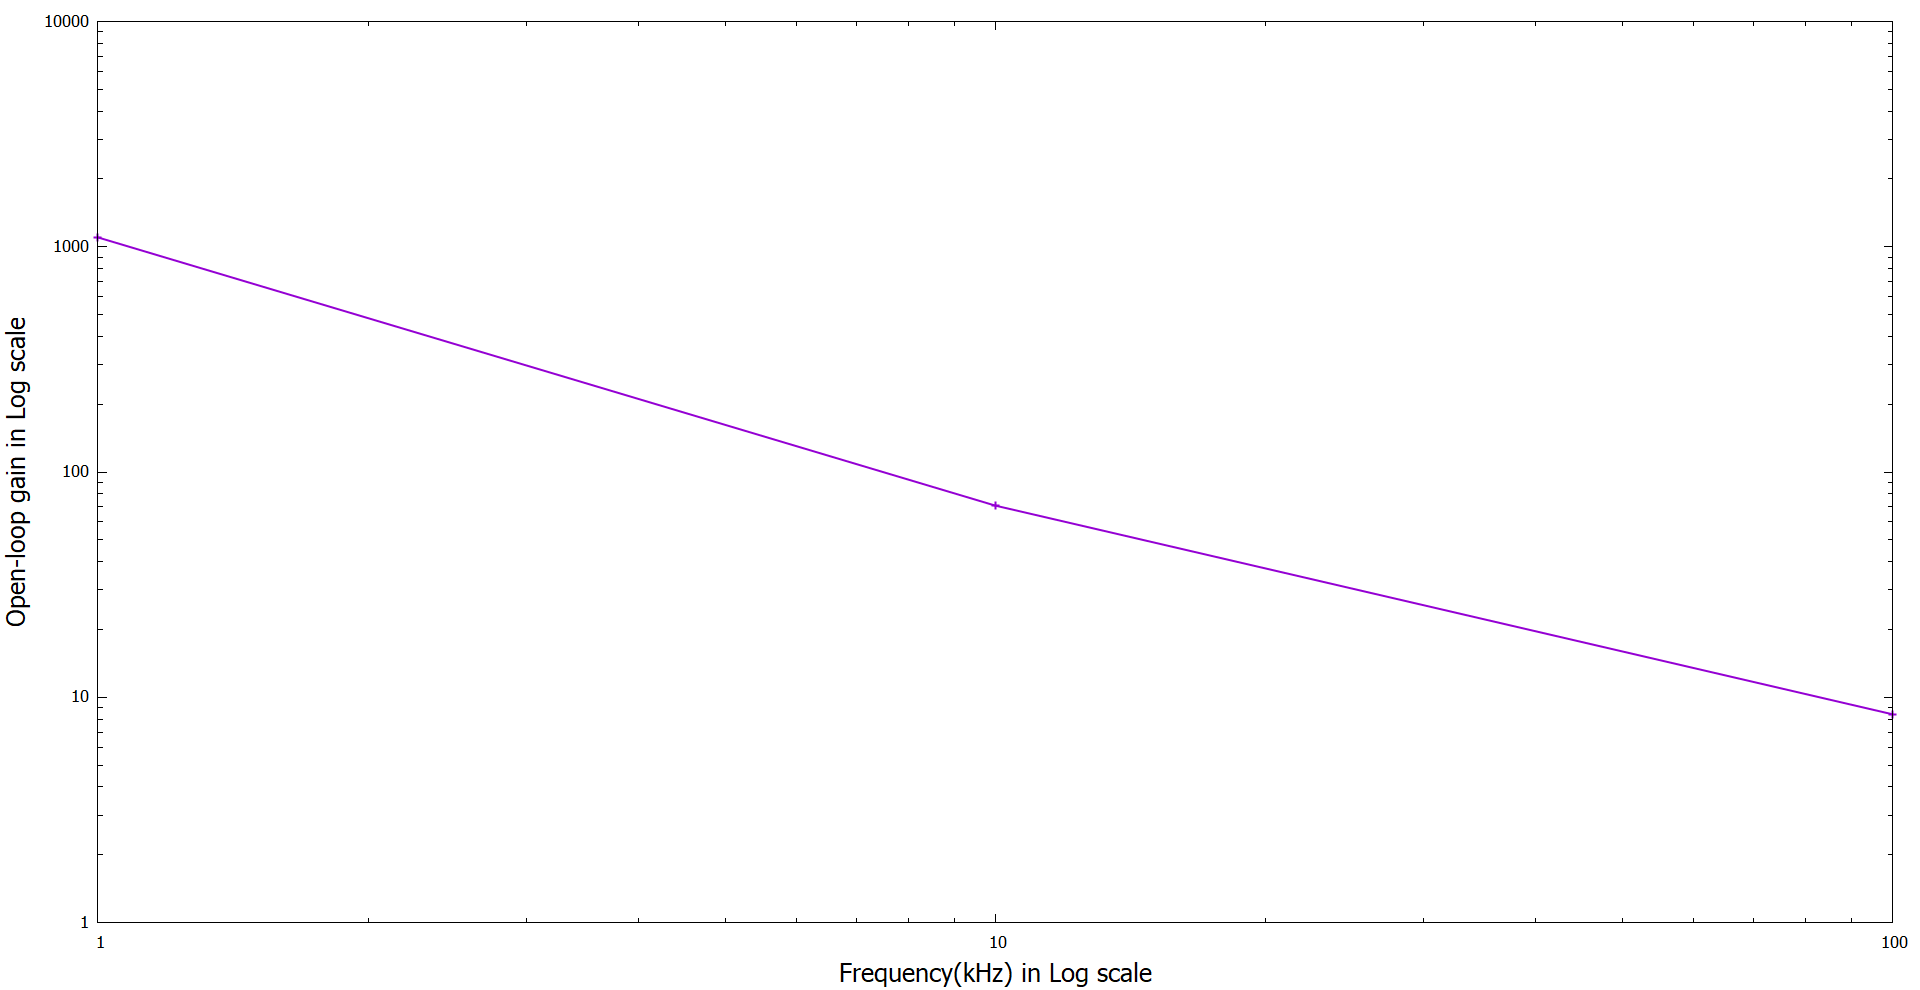
\includegraphics[width = \linewidth]{aLAB-2-1.png}
                \caption{$A_v$ Vs frequency in log scale}
            \end{subfigure}
            \begin{subfigure}{0.1\linewidth}
                \centering
                \begin{tabular}{|c|c|}
                   \hline
                     \bfseries frequency(kHz) & $\mathbf{A_v}$ \\ \hline
                     1  & 1100 \\ \hline
                     10  & 70.93 \\ \hline
                     100  & 8.4 \\ \hline
                \end{tabular}
            \end{subfigure}
        \end{figure}
        
\\
     This plot is linear and matches approximately with the open-loop gain vs frequency curve in log scale given in the datasheet of UA741.
        \begin{figure}[H]
            \centering
            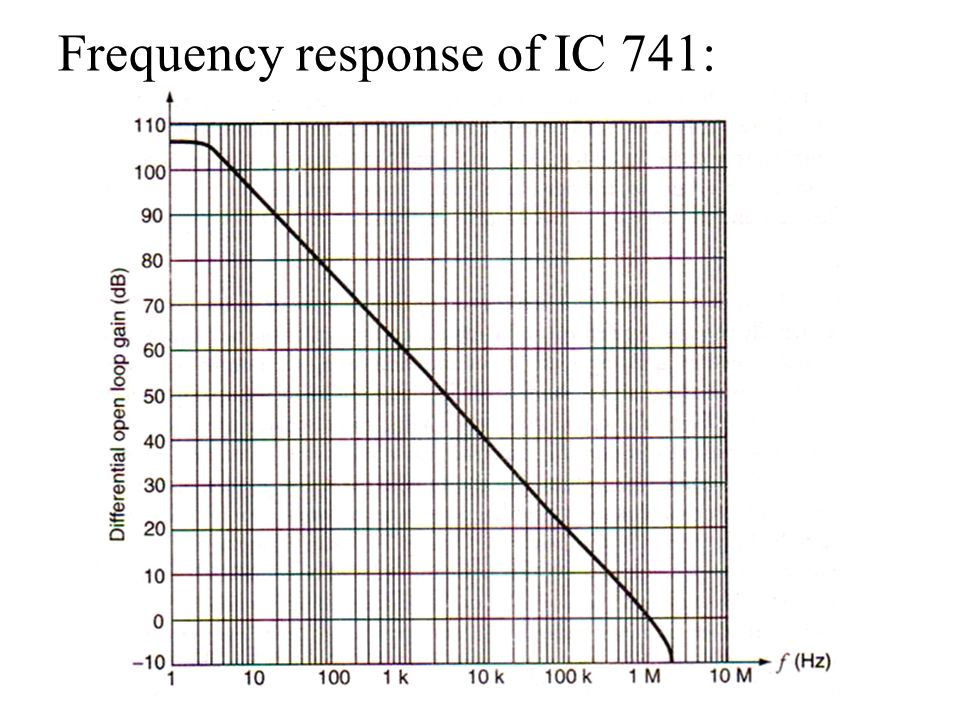
\includegraphics[width = 0.8\linewidth, height = 3in]{slide_14.jpg}
            \caption{Amplification v/s Frequency}
        \end{figure}

\section{Questions for reflection}

1. If the method for null-adjustment is as simple as the one you performed in lab, why isn't the 741 op-amp sold with the offset voltage internally calibrated?\\
\\
\textbf{Ans.} Some of the reasons could be:
    \begin{itemize}
        \item Input offset voltage value may change with temperature or age.
        \item Since offset voltage is itself generated because of manufacturing process, its value could not be known for sure.
        \item One cannot remove the offset voltage completely, it can be reduced to few microvolts.
    \end{itemize}
    That is why 741 op-amp isn't sold with the offset voltage internally calibrated.
\\\\
2. If the temperature in the lab were different from what it was when you performed the experiment, do you expect the pot value you ended up with will still give you offset nullification? Explain your answer. Hint: Look at the internal circuit diagram and figure out what parameters may change when the temperature changes.\\
\\
\textbf{Ans.}  No. With the change in temperature, offset voltage changes and hence the pot value required for offset nullification would change.
        \begin{figure}[H]
            \centering
            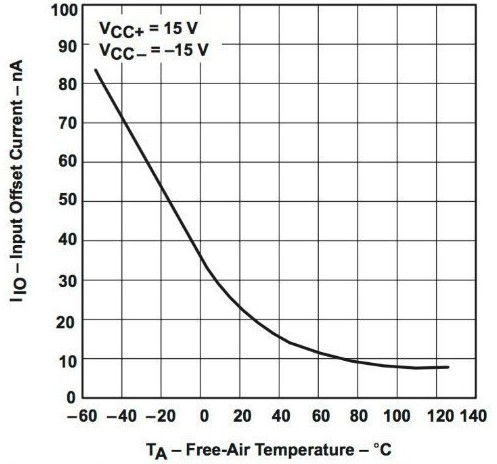
\includegraphics[width = 0.5\linewidth, height = 3in]{op.jpg}
            \caption{Input Offset Voltage v/s Temperature}
        \end{figure}
        
\\\\
3. What is the slew-rate of an op-amp? Read up the definition and explain it in your own words here. Could you suggest an experiment to measure slew-rate of op-amp 741?\\
\\
\textbf{Ans.} Slew-rate of an op-amp specifies the maximum and minimum limit of rate of change of voltage per unit of time i.e. when the input is amplified, the output cannot rise to a large value, because of the upper limit slew-rate specification of op-amp.
\\\\
We can use a non-inverting amplifier of gain one and give a square wave as input, as a square wave is discontinuous we expect the output to change it's value in infinitesimal time which is not observed practically because of slew rate. So the slew rate would be voltage of the top level of the distorted square output voltage signal divided by time taken to reach that level from bottom level. 
\\\\
\newpage
4. What is the role of capacitor C in the circuit you used in the second part of the lab (i.e. in figure 8 of the hand-out)? (Hint: there is a statement in the hand-out mentioning why C is connected; could you explain why that statement is true?)\\
\\
\textbf{Ans.} The capacitor C prevents the circuit from oscillating. We see that
coupled with R4 and R5, capacitor acts as an integrator. From the Bode plot
(shown in Figure 10) of capacitor we observe that capacitor filters out the
high frequency noise (which could have greatly affected in the measurement
of AOL)

        \begin{figure}[H]
            \centering
            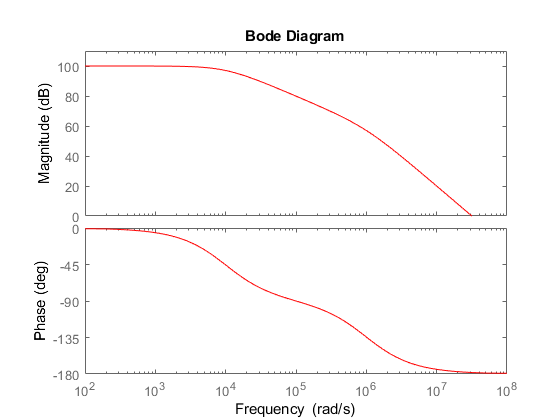
\includegraphics[width = 0.5\linewidth, height = 3in]{opampdemo_01.png}
            \caption{ Bode Plot of an Integrator}
        \end{figure}


\vspace{4cm}

    \begin{thebibliography}{9}

        \bibitem{Analog LAB Manual} 
        Non-idealities of op-amp File 
        \\\texttt{https://moodle.iitb.ac.in/mod/resource/view.php?id=92663}
        \bibitem{Datasheet of UA741}
        Datasheet of OpAmp UA741
        \\\texttt{https://www.slideshare.net/YongHeuiCho/u-a741}
        
    \end{thebibliography}

\end{document}

